%===============================================================================
% LaTeX sjabloon voor de bachelorproef toegepaste informatica aan HOGENT
% Meer info op https://github.com/HoGentTIN/latex-hogent-report
%===============================================================================

\documentclass[dutch,dit,thesis]{hogentreport}

\usepackage{lipsum} % For blind text, can be removed after adding actual content

%% Pictures to include in the text can be put in the graphics/ folder
\graphicspath{{../graphics/}}

%% For source code highlighting, requires pygments to be installed

%% Gebruik GEEN outputdir bij gebruik van de HOGENT Docker-container
\usepackage[chapter]{minted}
\usemintedstyle{solarized-light}

\setminted{%
    autogobble,
    frame=lines,
    breaklines,
    linenos,
    tabsize=4
}


%% Ensure the list of listings is in the table of contents
\renewcommand\listoflistingscaption{%
    \IfLanguageName{dutch}{Lijst van codefragmenten}{List of listings}
}
\renewcommand\listingscaption{%
    \IfLanguageName{dutch}{Codefragment}{Listing}
}

\renewcommand*\listoflistings{%
    \cleardoublepage\phantomsection\addcontentsline{toc}{chapter}{\listoflistingscaption}%
    \listof{listing}{\listoflistingscaption}%
}

%%---------- Document metadata -------------------------------------------------
\author{Tomas Boone}
\supervisor{Dhr. Bosteels}
\cosupervisor{Dhr. T. Vanhooren}
\title[Een Proof of Concept op Basis van NBB-Data]%
    {Big Data voor Kredietrisicoanalyse}
\academicyear{2023--2024} % Pas eventueel aan naar het huidige academiejaar
\examperiod{1}
\degreesought{\IfLanguageName{dutch}{Professionele bachelor in de toegepaste informatica}{Bachelor of applied computer science}}
\partialthesis{false} %% To display 'in partial fulfilment'
\institution{VDK Bank}

%% Add global exceptions to the hyphenation here
\hyphenation{back-slash}

%% The bibliography (style and settings are  found in hogentthesis.cls)
\addbibresource{bachproef.bib}            %% Bibliography file
\addbibresource{../voorstel/voorstel.bib} %% Bibliography research proposal
\defbibheading{bibempty}{}

%% Prevent empty pages for right-handed chapter starts in twoside mode
\renewcommand{\cleardoublepage}{\clearpage}
\renewcommand{\arraystretch}{1.2}

%% Content starts here.
\begin{document}

%---------- Front matter -------------------------------------------------------
\frontmatter

\hypersetup{pageanchor=false} %% Disable page numbering references

%% Generates title page content
\maketitle
\hypersetup{pageanchor=true}

%%=============================================================================
%% Voorwoord
%%=============================================================================

\chapter*{\IfLanguageName{dutch}{Woord vooraf}{Preface}}%
\label{ch:voorwoord}

Voor u ligt de bachelorproef ``Big Data voor Kredietrisicoanalyse: Een Proof of Concept op Basis van NBB-Data''. Dit werk vormt het sluitstuk van mijn opleiding Professionele Bachelor in de Toegepaste Informatica, afstudeerrichting AI \& Data Engineering, aan de HOGENT.

De keuze voor dit onderwerp kwam voort uit mijn sterke interesse in de financiële sector en de overtuiging dat er in de dataset van de Nationale Bank nog ongekende inzichten en analysemogelijkheden verborgen zitten. Het bouwen van een robuuste data-architectuur die ruwe financiële gegevens omzet in bruikbare, voorspellende inzichten, vormde een boeiende uitdaging waarin ik de opgedane academische theorie perfect aan de praktijk kon toetsen.

Ik wens graag een aantal personen te bedanken die hebben bijgedragen tot de totstandkoming van deze bachelorproef. In de eerste plaats gaat mijn dank uit naar mijn co-promotor, dhr.\ T.\ Vanhooren, voor de waardevolle feedback, de professionele begeleiding en de mogelijkheid om dit onderzoek uit te voeren. Daarnaast wil ik ook mijn promotor, dhr. Bosteels, bedanken voor de kritische sturing en de academische ondersteuning tijdens het schrijfproces. Ten slotte bedank ik mijn familie en vrienden voor hun onvoorwaardelijke steun tijdens mijn studies.

Ik wens u veel leesplezier.

Tomas Boone,\\
Gent, juni 2024
%%=============================================================================
%% Samenvatting
%%=============================================================================

\chapter*{\IfLanguageName{dutch}{Samenvatting}{Abstract}}



%---------- Inhoud, lijst figuren, ... -----------------------------------------
\tableofcontents
\listoffigures
\listoftables
\listoflistings

%---------- Kern ---------------------------------------------------------------

\mainmatter{}

%%=============================================================================
%% Inleiding
%%=============================================================================

\chapter{\IfLanguageName{dutch}{Inleiding}{Introduction}}%
\label{ch:inleiding}

Bij het toekennen van zakelijke leningen staan banken en kredietverstrekkers voor de uitdaging om een nauwkeurige inschatting te maken van het risico op wanbetaling. Om gefundeerde beslissingen te nemen rond rentevoeten en looptijden, analyseren financiële risicoanalisten en beleidsmakers de financiële gezondheid van een aanvragende onderneming. Analisten baseren zich in de huidige praktijk voornamelijk op de meest recente jaarrekening van de specifieke onderneming, vaak aangevuld met externe credit scores. Deze traditionele aanpak focust zich sterk op individuele dossiers, waardoor het grote plaatje soms ontbreekt.

\section{\IfLanguageName{dutch}{Probleemstelling}{Problem Statement}}%
\label{sec:probleemstelling}

De huidige werkwijze voor financiële risicoanalyse is overwegend reactief. Door sterk te focussen op individuele, historische jaarrekeningen, isoleert het traditionele proces de onderneming van haar bredere sectorale context \autocite{Qiang2024}. Een bedrijf presteert immers nooit in een vacuüm; de financiële gezondheid hangt nauw samen met sectorbrede economische verschuivingen \autocite{Bhattarai2024}. Het handmatig vergelijken van de cijfers van een onderneming met al haar sectorgenoten vormt echter een enorm arbeidsintensief proces, zeker zonder de juiste technologische ondersteuning. Bijgevolg zien analisten sectorbrede trends en vroegtijdige waarschuwingssignalen voor wanbetaling vaak over het hoofd \autocite{Bhattarai2024}. Zoals \textcite{Moscato2021} aangeven, leidt dit gebruik van traditionele en statische methoden vaak tot een suboptimale risico-inschatting, wat aanzienlijke financiële verliezen voor de kredietverstrekker met zich mee kan brengen.
\section{\IfLanguageName{dutch}{Onderzoeksdoelstelling}{Research objective}}%
\label{sec:onderzoeksdoelstelling}

Dit onderzoek heeft als doel de kredietverleningsprocessen binnen banken te optimaliseren door middel van datagedreven technologieën. Het concrete eindresultaat is de ontwikkeling van een Proof of Concept (PoC). Binnen deze PoC verzamelt een geautomatiseerde pijplijn de volledige dataset van de Nationale Bank van België (NBB) van de afgelopen drie jaar, om deze vervolgens in te laden in een schaalbare database. De opzet fungeert als fundament voor experimenten rond sectorbrede benchmarking en predictieve analyses, om te testen of dergelijke methoden een aantoonbare meerwaarde bieden bovenop de klassieke dossierbehandeling.

\section{\IfLanguageName{dutch}{Onderzoeksvraag}{Research question}}%
\label{sec:onderzoeksvraag}

Om tegemoet te komen aan de probleemstelling en de doelstelling te behalen, hanteert dit onderzoek de volgende centrale onderzoeksvraag:

\begin{displayquote}
In welke mate kan een Big Data-architectuur op basis van publiekelijk beschikbare data bijdragen tot een nauwkeurigere financiële risico-inschatting bij kredietverlening?
\end{displayquote}

Om deze centrale vraag te structureren en systematisch te beantwoorden, formuleert het onderzoek volgende deelvragen:
\begin{enumerate}
    \item Hoe kunnen we de dataset (gratis) opzetten zodat deze bruikbaar is voor verdere data analyse?
    \item Welke factoren bepalen een zinvolle segmentatie of clustering van ondernemingen om een representatieve sector-benchmark te bekomen?
    \item Welke machine learning-modellen zijn geschikt om op basis van historische financiële ratio's toekomstige bedrijfsprestaties te voorspellen?
    \item Welke impact heeft het implementeren van een Big Data-platform op de werkwijze van de financiële analist? Kunnen deze nieuwe modellen helpen om een bedrijf te scoren?
\end{enumerate}


\section{\IfLanguageName{dutch}{Opzet van deze bachelorproef}{Structure of this bachelor thesis}}%
\label{sec:opzet-bachelorproef}

De rest van deze bachelorproef is als volgt opgebouwd:

In Hoofdstuk~\ref{ch:stand-van-zaken} volgt een uitgebreid literatuuroverzicht dat de stand van zaken binnen de traditionele ratio-analyse, beschikbare softwareoplossingen en de technologische verschuivingen naar Big Data en Machine Learning in kaart brengt. In Hoofdstuk~\ref{ch:methodologie} verantwoordt de tekst de gekozen onderzoeksstrategie en beschrijft het de vier fasen van de proof of concept.

Vervolgens documenteert Hoofdstuk~\ref{ch:architectuur} de technische architectuur, de inrichting van het cloud-datawarehouse en de werking van de ETL-pijplijn. Hoofdstuk~\ref{ch:resultaten} evalueert daarna de verzamelde resultaten, met bijzondere aandacht voor de exploratieve sectoranalyse en de accuraatheid van de predictieve machine learning-modellen.

In Hoofdstuk~\ref{ch:conclusie}, ten slotte, geeft het onderzoek een sluitend antwoord op de onderzoeksvragen, bediscussieert het de relevantie van de bevindingen voor de financiële sector en reikt het suggesties aan voor vervolgonderzoek.

\chapter{\IfLanguageName{dutch}{Stand van zaken}{State of the art}}%
\label{ch:stand-van-zaken}

Dit hoofdstuk schetst het theoretisch kader voor het evalueren van kredietrisico's en de rol van datatechnologie daarin. Om de centrale onderzoeksvraag te kunnen beantwoorden, analyseert de literatuurstudie eerst de traditionele methodieken rond kredietrisicoanalyse en de beperkingen van de huidige softwareoplossingen. Vervolgens verschuift de focus naar de technologische context, waarbij de mogelijkheden van cloud-datawarehouses en machine learning-algoritmen (ML) binnen de financiële sector (FinTech) worden belicht.

\section{Traditionele Risicoanalyse en Bestaande Software}

De financiële gezondheid van een onderneming evalueert men traditioneel aan de hand van ratio-analyse. Analisten berekenen indicatoren zoals liquiditeit, solvabiliteit en rentabiliteit op basis van de neergelegde jaarrekeningen \autocite{Ooghe2021}. Modellen, zoals de Altman Z-score, proberen op basis van deze ratio's de kans op een eventueel faillissement te voorspellen.

Om dit proces efficiënter te maken voor de analist, biedt de markt diverse softwaretoepassingen aan, waaronder Companyweb, Belfirst en OpenTheBox. Deze platformen slagen erin bedrijfsstructuren te visualiseren en geven toegang tot sectorgemiddelde ratio's. Hoewel deze tools uitstekend presteren voor het raadplegen van individuele klantdossiers, missen ze vaak de flexibiliteit om grootschalige, op maat gemaakte predictieve modellering uit te voeren op ruwe data. Gebruikers zijn gebonden aan de visualisaties en berekeningen die de softwareleverancier voorziet, wat exploratieve analyse op grotere schaal belemmert.

\section{Big Data en Cloud Computing in FinTech}

De opkomst van 'FinTech' brengt een verschuiving teweeg van statische analyses naar dynamische, datagedreven toepassingen. Binnen dit domein zijn cloud-native datawarehouses cruciaal. Architecturen zoals Google BigQuery vertonen superieure prestaties bij het verwerken van datasets met miljoenen rijen in vergelijking met traditionele, on-premise servers \autocite{Gupta2024}. BigQuery typeert zich door een serverless opbouw en laat toe om complexe data analyses uit te voeren op een kostenefficiënte en uiterst performante manier \autocite{ActiveViam2025}.

% (Deel 1 en 2 blijven behouden zoals je had, hier is de correctie vanaf sectie 3) ...

\section{Machine Learning voor Kredietrisico}

Naast de opslag en verwerking van Big Data, besteedt de literatuur veel aandacht aan de inzet van Machine Learning voor het voorspellen van kredietrisico's. Recente studies tonen aan dat moderne datagedreven technieken aanzienlijk beter kunnen presteren dan traditionele rekenmethodes. Volgens \textcite{Moscato2021} bieden vooral geavanceerde algoritmen, zoals ensemble learning, een hogere accuraatheid bij \textit{credit scoring}. De integratie van zulke ML-technieken, gecombineerd met de rekenkracht van cloud-datawarehouses en gestructureerde datasets zoals die van de Nationale Bank van België, kan hierdoor nieuwe perspectieven bieden voor een proactiever en nauwkeuriger acceptatiebeleid in de kredietverlening.

Een kritieke factor bij de ontwikkeling van financieel voorspellende machine learning-modellen is de kwaliteit en structuur van de trainingsdataset. Het gebruik van één generiek model om de financiële ratio's van alle ondernemingen te voorspellen, levert doorgaans onnauwkeurige resultaten op wegens de grote onderlinge absolute verschillen en marktdynamieken. Er moet bijgevolg per financieel zinvolle cluster een specifiek model worden ontwikkeld om de voorspellingen binnen de cluster (intra-cluster) te optimaliseren.

In de academische literatuur worden doorgaans twee methoden onderscheiden om deze clusters op te bouwen: een handmatige segmentatie op basis van vooraf gedefinieerde parameters, of een algoritmische clustering (zoals K-means). Binnen de traditionele segmentatie zijn de voornaamste determinanten voor het groeperen van ondernemingen reeds afgebakend. Ten eerste vormt de grootte van de onderneming een fundamentele variabele; \textcite{cultrera2016} stellen immers dat grotere bedrijven (die het volledig schema hanteren) profiteren van schaalvoordelen, een vlottere toegang hebben tot bankkredieten en een totaal ander werkkapitaalbeheer hanteren dan micro-ondernemingen. Een micro-entiteit wordt bovendien vaak gestuurd door de persoonlijke financiën van de zaakvoerder (bijv. via de rekening-courant), wat de solvabiliteitsratio's scheeftrekt vergeleken met een grote NV. Een algoritme dat deze profielen door elkaar haalt, leert patronen aan die in realiteit niet bestaan.

Ten tweede is de leeftijd (de levenscyclus) van de onderneming een bepalende factor, waarbij \textcite{cho2020} aantonen dat het voorspellend vermogen toeneemt wanneer modellen worden afgestemd op de maturiteit van de entiteit. Tot slot is een sectoriële afbakening noodzakelijk, aangezien financiële structuren sterk fluctueren naargelang de kernactiviteit en het gebruik van deze afbakening een significante en bewezen impact heeft op de accuraatheid van insolventiemodellen \autocite{tian2017}.

Aan de andere kant toont recent onderzoek aan dat algoritmische clusteringtechnieken in staat zijn om meer homogene groepen te vormen dan deze traditionele opsplitsingsmethoden. Door hun datagedreven, \textit{unsupervised} karakter kunnen dergelijke algoritmen complexe, onderliggende patronen in de data identificeren, zonder daarbij afhankelijk te zijn van rigide, vooraf bepaalde labels \autocite{hou2016financial, gulal2023predicting, zhao2024boosting}.toont aan dat clusteringtechnieken in staat zijn om meer homogene groepen te vormen dan traditionele opsplitsingsmethoden. Door hun datagedreven, \textit{unsupervised} karakter kunnen deze algoritmen complexe, onderliggende patronen in de data identificeren, zonder daarbij afhankelijk te zijn van rigide, vooraf bepaalde labels \cite{hou2016financial, gulal2023predicting, zhao2024boosting}.
%%=============================================================================
%% Methodologie
%%=============================================================================

\chapter{\IfLanguageName{dutch}{Methodologie}{Methodology}}%
\label{ch:methodologie}

Dit onderzoek volgt de methodologie van \textit{design science research} (constructief onderzoek). Bij deze aanpak ontwikkelt en evalueert de onderzoeker een Proof of Concept (PoC) bestaande uit een cloud-architectuur en predictieve modellen met doel een concreet probleem uit de praktijk op te lossen. De technologische realisatie steunt voornamelijk op Google Cloud Platform (waaronder Cloud Storage en BigQuery) vanwege de serverless architectuur, lage kosten en hoge performantie \autocite{GoogleCloud2024}. Voor de datamanipulatie en modeltraining wordt gebruikgemaakt van de programmeertaal Python.

Het onderzoek verloopt gestructureerd via vier grote fasen.

\section{Fase 1: Data Ingestie en Engineering}
In de eerste fase verkrijgt het onderzoek data van de Nationale Bank van België (NBB) via het Open Data portaal. Om deze ongestructureerde of ruwe data bruikbaar te maken, ontwikkelt het onderzoek een eigen ETL-pipeline (Extract, Transform, Load). Deze pipeline garandeert volledige controle over de structuur van de data. Een opgeschoonde dataset vormt de absolute vereiste om in latere stappen sectoren correct te classificeren en algoritmen effectief te trainen.

\section{Fase 2: Groepering en Segmentatie}
Tijdens de tweede fase clustert de PoC de ondernemingen in financieel gelijkaardige groepen. De initiële classificatie gebeurt op basis van NACE-codes, wat toelaat om bedrijven binnen een specifieke markt af te lijnen. Het onderzoek analyseert tevens welke bijkomende variabelen, zoals bedrijfsgrootte of regio, in rekening gebracht moeten worden om tot een zo zinvol mogelijke segmentatie te komen.

\section{Fase 3: Empirische Studie}
Na het groeperen volgt een empirische studie van de data in de geconstrueerde omgeving. Door oppervlakkige trends in kaart te brengen en te valideren aan de hand van bestaande financiële intuïtie, controleert deze fase de validiteit van de data. Deze exploratieve analyse helpt bij het identificeren van ontbrekende waarden en vormt de basis voor het definiëren van de parameters (features) voor het predictieve model.

\section{Fase 4: Voorspellende Analyse}
In de laatste fase configureert en traint het onderzoek per segment een Machine Learning-model. Dit gebeurt met behulp van frameworks zoals BigQuery ML en scikit-learn. De doelstelling hierbij is om op basis van de historische financiële prestaties (bijvoorbeeld het jaar X-2 en X-1) de kritieke ratio's of het risicoprofiel voor jaar X te voorspellen. Ten slotte toetst de onderzoeker de accuraatheid van deze modellen af om te bepalen in welke mate historische NBB-data voldoende voorspellende waarde bevatten.
%%=============================================================================
%% Architectuur en Implementatie
%%=============================================================================

\chapter{\IfLanguageName{dutch}{Architectuur en Implementatie}{Architecture and Implementation}}%
\label{ch:architectuur}

Dit hoofdstuk beschrijft de technische realisatie van de Proof of Concept (PoC). Om de afhankelijkheid van statische kredietanalyses te doorbreken, werd een schaalbare cloud-architectuur ontworpen. De focus ligt op het automatiseren van de data-ingestie en het voorbereiden van de dataset voor latere machine learning-toepassingen.



\begin{figure}
    \centering
    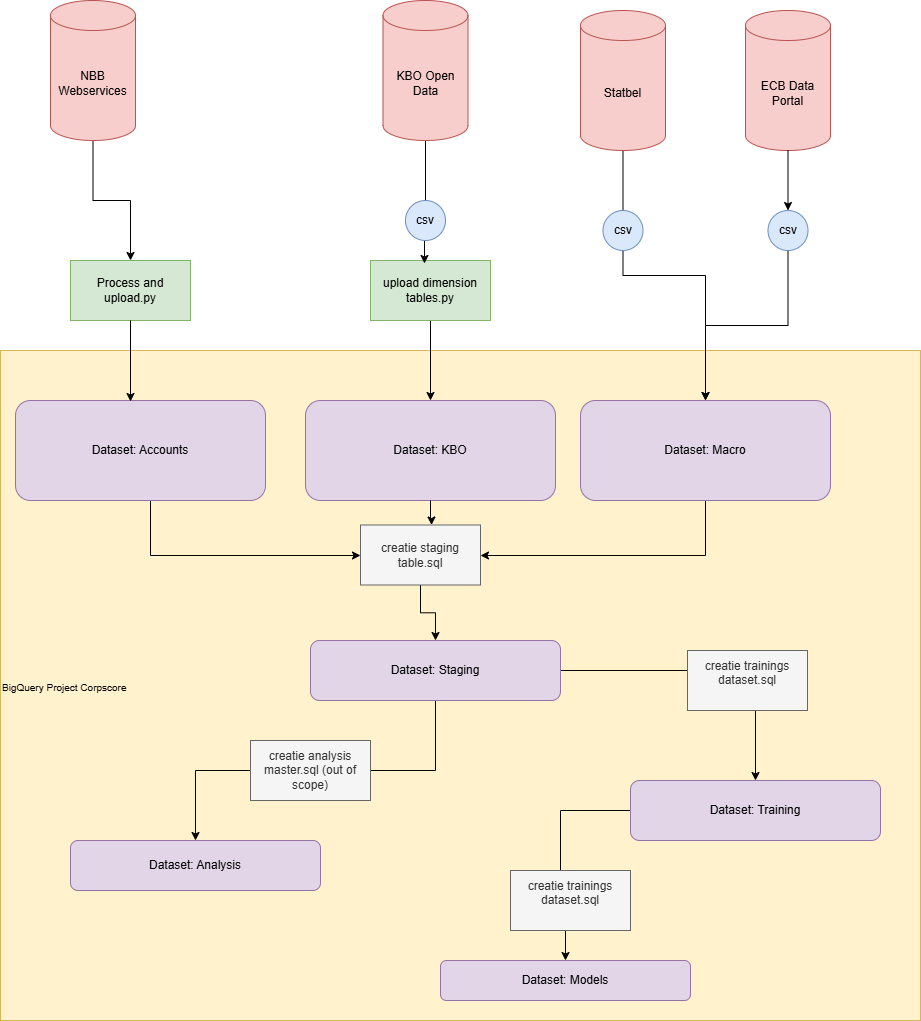
\includegraphics{images/Project flow.drawio}
    \caption{}
    \label{fig:project-flow.drawio}
\end{figure}


%%=====tables/model_metrics_heulistic_seg==================================
%% Resultaten
%%=============================================================================

\chapter{\IfLanguageName{dutch}{Resultaten en Evaluatie}{Results and Evaluation}}%
\label{ch:resultaten}

Dit hoofdstuk presenteert de bevindingen van de geconstrueerde Proof of Concept. Een evaluatie van de geïmplementeerde predictieve machine learning-modellen voor de verschillende segmentatie methoden. Ook wordt geconcludeerd wat nog moet gebeuren voor een meerwaarde in het werkveld te bieden.

\section{Data Ingestie}
Hoe kunnen we de data, beschikbaar via het NBB portaal, in een geschikte vorm verkrijgen? De nationale bank van België voorziet verschillende webservices om digitaal te interageren met hun data.
Voor het extraheren van grote hoeveelheden data is er een bulk API beschikbaar, die alle neerleggingen, ingediend op één bepaalde dag, terug geeft in een handig JSON formaat.
Helaas ontrbeekt hier een ondernemingsnummer waardoor deze data nagenoeg nutteloos wordt voor verdere analyse.
Dan blijft enkel de single API over, die per ondernemingsnummer alle beschikbare neergelegde documenten terug geeft. Deze blijt wel over alle nodige data te beschikken maar moet één voor één aangeroepen worden.
Een asynchroon script bleek hier een (weinig performante), maar geschikte oplossing voor een beperkt aantal jaren.
Welk platform gebruiken voor verdere tranformaties en analyses? BigQuery bleek heel geschikt voor de opslag en tranformaties van grote hoeveelheden data, terwijl de kosten heel laag bleven.

\section{Heulistische Segmentatie}
Levert een op regels gebaseerd (heuristische) segmentatie betere resultaten op dan een clustering algoritme (k-means)?
Deze segmentatie methodes werden ontwikkeld met het doel een nuttig machine learning algoritme te trainen voor krediet scoring.
De evaluatie van deze methodes is dan ook gelijk gesteld aan de evalutatie van hun resulterende modellen.
Hoeveel segmenten? Heulistische segmentatie op basis van nace code, grootte en model type leverde maar liefst 6314 segmenten op. Dit resulteert in te weinig data per segment, we moeten minder specifiek gaan.
We namen enkele sectoren en modeltypes samen. Zo bekomen we nog 32 groepen waarvan de grootste voldoende data hebben voor een modeltraining.
\linebreak
Als benchmark trainen we een XGBoost model zonder segmentatie. Dit zal uiteindelijk zelf segmenteren. We bekomen volgende resultaten:
\begin{table}[htbp]
    \small
    \caption{XGBoost model metrics zonder voorafgaande segmentatie}
    \label{tab:model_metrics_no_seg}
    \begin{tabular}{llllllllllllll}
    \toprule

    \textbf{trial id} &
    \textbf{precision} &
    \textbf{recall} &
    \textbf{accuracy} &
    \textbf{f1 score} &
    \textbf{log loss} &
    \textbf{roc auc} \\
    \midrule

    \multicolumn{1}{l}{1} &
    \multicolumn{1}{r}{0.6276} &
    \multicolumn{1}{r}{0.8838} &
    \multicolumn{1}{r}{0.8917} &
    \multicolumn{1}{r}{0.7340} &
    \multicolumn{1}{r}{0.2662} &
    \multicolumn{1}{r}{0.9586} \\
    \bottomrule

\end{tabular}

\end{table}

Volgende paramaters blijken het meeste effect op de accuracy score te hebben:

\begin{table}[htbp]
    \small
    \caption{Feature importance XGBoost model zonder voorafgaande segmentatie}
    \label{tab:feature_importance_no_seg}
    \begin{tabular}{lrr} % l=links, r=rechts (cijfers staan best rechts voor leesbaarheid)
    \toprule
    \textbf{feature}      & \textbf{importance weight} & \textbf{importance gain} \\
    \midrule
    solvency\_y2          & 78.00                        & 1,382.15                   \\
    liquidity\_custom\_y2 & 50.00                        & 638.79                     \\
    equity\_y2            & 114.00                       & 294.75                     \\
    debt\_to\_equity\_y2  & 60.00                        & 181.28                     \\
    roa\_y2               & 58.00                        & 169.90                     \\
    raw\_model\_type      & 74.00                        & 116.58                     \\
    roe\_y2               & 94.00                        & 72.23                      \\
    net\_profit\_y2       & 42.00                        & 49.34                      \\
    equity\_y1            & 38.00                        & 49.23                      \\ % <--- De extra \\ hier lost de error op
    \bottomrule
\end{tabular}
\end{table}

Om te zien of voorafgaande sgemtnatie effect heeft en welke methode de beste is, maakten we gebruik van stratified modeling. We namen de 3 grootste segmenten en trainden hier 3 individuele (in tegenstelling to 1 globaal) XGBoost model op.
Dit waren onze top 3 sectoren (heulistisch gesegmenteerd):
\begin{itemize}
    \item \textbf{diensten/micro}: Deze sector omvat consultancy, it-diensten, enz.
    \item \textbf{handel/micro}: Kleinere winkels en retail.
    \item \textbf{bouw/micro}: Kleinere bouwbedrijven: een kleine loodgieter of aannemer.
  \end{itemize}

Onze drie XGBoostmodellen toonden hogere gemiddelde scores:

\begin{table}[htbp]
    \small
    \caption{XGBoost model metrics na sectorale segmentatie (enkel micro ondernemingen)}
    \label{tab:model_metrics_heul_seg}
    \begin{tabular}{lrrrrrr}
    \toprule
    \textbf{sector} & \textbf{precision} & \textbf{recall} & \textbf{accuracy} & \textbf{f1\_score} & \textbf{log\_loss} & \textbf{roc\_auc} \\
    \midrule
    \textbf{diensten} & 0.6826 & 0.8753 & 0.9333 & 0.7670 & 0.1957 & 0.9711 \\
    \textbf{handel}   & 0.7155 & 0.8507 & 0.9388 & 0.7773 & 0.1998 & 0.9688 \\
    \textbf{bouw}     & 0.7136 & 0.8391 & 0.9375 & 0.7713 & 0.1990 & 0.9665 \\
    \bottomrule
\end{tabular}
\end{table}

een beduidende verbetering op de benchmark. Verrassend want wanneer we naar de feature importance kijken van het base model zien we dat model type en sector redelijk laag staan (respectievelijk plaats 7 en 49). Dit betekent dat ze normaal weinig invloed zouden mogen hebben op de resultaten.
Toen je alles op één grote hoop gooide, moest XGBoost constant compromissen sluiten. Een liquiditeitsratio van 0.9 is voor een IT-consultant met enkel debiteuren (Zakelijke Diensten) misschien geen direct probleem, maar voor een aannemer wél. Door het algoritme nu exclusief te trainen op IT'ers en consultants (Micro/Micro), hebben de beslissingsbomen hyper-specifieke regels kunnen ontdekken die puur voor díe sector gelden. De "ruis" van de andere sectoren is weg.

\section{K-means Segmentatie}
De eerste segmentatie op nagenoeg alle data bracht de ondernemingen allemaal samen in 1 bucket; Dit kwam door de grote hoeveelheid ongestandaardizeerde data.
Bij een tweede poding werden enkel belangrijke ratio's weerhouden. Deze werden gewinsorizeerd om extreme uitschieters te normalizeren.
\begin{figure}[htbp]
    \centering
    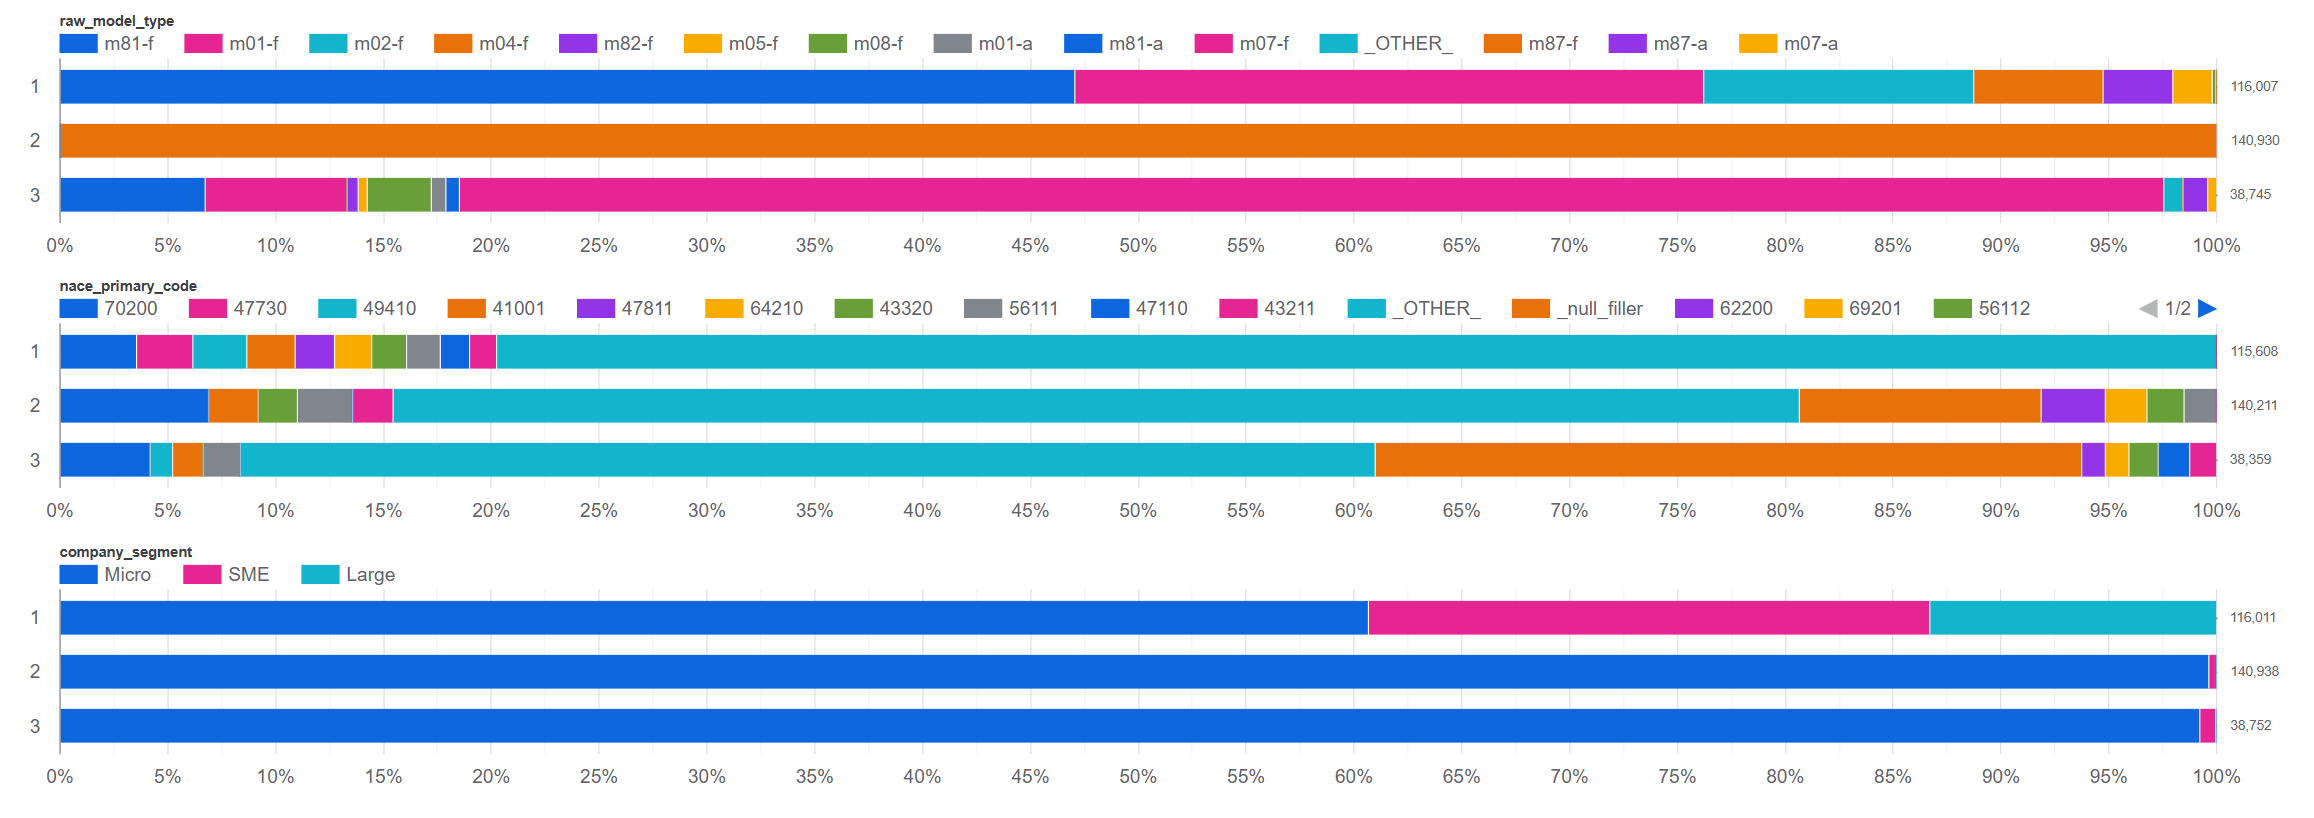
\includegraphics[width=\textwidth]{images/cluster-categories}
    \caption{Verdeling van de verschillende categorische parameters in de clusters}
    \label{fig:cluster-cats}
\end{figure}


\begin{table}[ht]
    \centering
    \caption{K-means Cluster Features}
    \label{tab:features_k_means}
    \resizebox{\textwidth}{!}{ % Dit dwingt de tabel naar de breedte van je tekst
        \begin{table}[ht]
    \centering
    \caption{Overzicht van K-means Centroids en Features (Gefilterd op >5000 ondernemingen)}
    \label{tab:features_k_means}
    \setlength{\tabcolsep}{2pt} % Verkleint de ruimte tussen kolommen om alles te laten passen
    \begin{tabularx}{\textwidth}{@{} r *{10}{X} r @{}}
        \toprule
        \textbf{ID} & \textbf{Rev\_y2} & \textbf{Equity} & \textbf{Profit\_y1} & \textbf{Profit\_y2} & \textbf{$\Delta$Rev} & \textbf{$\Delta$Cust} & \textbf{$\Delta$Inv} & \textbf{$\Delta$Liq\_C} & \textbf{$\Delta$Liq\_S} & \textbf{$\Delta$Supp} & \textbf{Count} \\
        \midrule
        \footnotesize \textbf{9} & 
        \cellcolor[HTML]{F9FCFA}\footnotesize 18.82 & 
        \cellcolor[HTML]{FFFFFF}\footnotesize 106k & 
        \cellcolor[HTML]{FFFFFF}\footnotesize 15k & 
        \cellcolor[HTML]{FFFFFF}\footnotesize 14k & 
        \cellcolor[HTML]{FCFEFD}\footnotesize -6.24 & 
        \cellcolor[HTML]{FDFFFE}\footnotesize -332 & 
        \cellcolor[HTML]{E0F3E9}\footnotesize -1.51 & 
        \footnotesize -0.32 & 
        \cellcolor[HTML]{A8DCC2}\footnotesize 0.38 & 
        \cellcolor[HTML]{F3FBF7}\footnotesize -10.92 & 
        \footnotesize 90163 \\
        
        \footnotesize \textbf{23} & 
        \cellcolor[HTML]{FBFDFC}\footnotesize 18.99 & 
        \cellcolor[HTML]{FAFDFC}\footnotesize 629k & 
        \cellcolor[HTML]{F8FDFA}\footnotesize 82k & 
        \cellcolor[HTML]{F7FCFA}\footnotesize 86k & 
        \cellcolor[HTML]{FEFFFE}\footnotesize -6.30 & 
        \cellcolor[HTML]{FEFFFE}\footnotesize -336 & 
        \cellcolor[HTML]{E0F3E9}\footnotesize -1.52 & 
        \footnotesize -0.24 & 
        \cellcolor[HTML]{FFFFFF}\footnotesize -12.52 & 
        \cellcolor[HTML]{F3FBF7}\footnotesize -10.94 & 
        \footnotesize 44377 \\

        \footnotesize \textbf{10} & 
        \cellcolor[HTML]{E9F6EF}\footnotesize 17.74 & 
        \cellcolor[HTML]{FFFFFF}\footnotesize 156k & 
        \cellcolor[HTML]{FFFFFF}\footnotesize 10k & 
        \cellcolor[HTML]{FFFFFF}\footnotesize 9k & 
        \cellcolor[HTML]{F5FBF8}\footnotesize -5.98 & 
        \cellcolor[HTML]{F9FDFB}\footnotesize -315 & 
        \cellcolor[HTML]{E3F4EB}\footnotesize -2.13 & 
        \footnotesize -0.14 & 
        \cellcolor[HTML]{B8E3CE}\footnotesize -2.07 & 
        \cellcolor[HTML]{F3FBF7}\footnotesize -10.92 & 
        \footnotesize 25842 \\

        \footnotesize 32 & 
        \cellcolor[HTML]{F0F9F5}\footnotesize 18.25 & 
        \cellcolor[HTML]{F3FAF7}\footnotesize 1.4M & 
        \cellcolor[HTML]{F6FCF9}\footnotesize 109k & 
        \cellcolor[HTML]{F6FCF9}\footnotesize 103k & 
        \cellcolor[HTML]{F8FCFA}\footnotesize -6.08 & 
        \cellcolor[HTML]{FFFFFF}\footnotesize -342 & 
        \cellcolor[HTML]{E7F5EE}\footnotesize -2.96 & 
        \footnotesize -0.03 & 
        \cellcolor[HTML]{ACDEC6}\footnotesize -0.32 & 
        \cellcolor[HTML]{F3FBF7}\footnotesize -10.93 & 
        \footnotesize 20178 \\

        \footnotesize 30 & 
        \cellcolor[HTML]{FBFDFC}\footnotesize 18.97 & 
        \cellcolor[HTML]{FFFFFF}\footnotesize 106k & 
        \cellcolor[HTML]{FFFFFF}\footnotesize 13k & 
        \cellcolor[HTML]{FFFFFF}\footnotesize 15k & 
        \cellcolor[HTML]{FDFEFD}\footnotesize -6.25 & 
        \cellcolor[HTML]{F0F9F5}\footnotesize -279 & 
        \cellcolor[HTML]{DAF0E6}\footnotesize -0.36 & 
        \footnotesize -0.28 & 
        \cellcolor[HTML]{9CD7BA}\footnotesize 2.14 & 
        \cellcolor[HTML]{FFFFFF}\footnotesize -11.65 & 
        \footnotesize 15901 \\

        \footnotesize 26 & 
        \cellcolor[HTML]{F6FBF8}\footnotesize 18.62 & 
        \cellcolor[HTML]{DFF2E9}\footnotesize 3.5M & 
        \cellcolor[HTML]{E6F5ED}\footnotesize 276k & 
        \cellcolor[HTML]{E3F4EC}\footnotesize 286k & 
        \cellcolor[HTML]{B6E2CD}\footnotesize -3.75 & 
        \cellcolor[HTML]{57BB8A}\footnotesize 335.15 & 
        \cellcolor[HTML]{D8F0E4}\footnotesize 0.15 & 
        \footnotesize -0.03 & 
        \cellcolor[HTML]{A9DCC3}\footnotesize 0.19 & 
        \cellcolor[HTML]{D2EDE0}\footnotesize -8.95 & 
        \footnotesize 15211 \\

        \footnotesize 18 & 
        \cellcolor[HTML]{57BB8A}\footnotesize 7.80 & 
        \cellcolor[HTML]{57BB8A}\footnotesize 18M & 
        \cellcolor[HTML]{57BB8A}\footnotesize 1.7M & 
        \cellcolor[HTML]{57BB8A}\footnotesize 1.6M & 
        \cellcolor[HTML]{57BB8A}\footnotesize -0.37 & 
        \cellcolor[HTML]{9ED8BC}\footnotesize 50.79 & 
        \cellcolor[HTML]{57BB8A}\footnotesize 27.38 & 
        \footnotesize 0.15 & 
        \cellcolor[HTML]{A9DDC4}\footnotesize 0.14 & 
        \cellcolor[HTML]{57BB8A}\footnotesize -1.76 & 
        \footnotesize 14411 \\

        \footnotesize 27 & 
        \cellcolor[HTML]{FFFFFF}\footnotesize 19.22 & 
        \cellcolor[HTML]{FFFFFF}\footnotesize 162k & 
        \cellcolor[HTML]{FDFFFE}\footnotesize 32k & 
        \cellcolor[HTML]{FDFEFE}\footnotesize 34k & 
        \cellcolor[HTML]{FFFFFF}\footnotesize -6.36 & 
        \cellcolor[HTML]{FFFFFF}\footnotesize -339 & 
        \cellcolor[HTML]{E2F4EB}\footnotesize -1.96 & 
        \footnotesize -0.35 & 
        \cellcolor[HTML]{A0D9BD}\footnotesize 1.55 & 
        \cellcolor[HTML]{F3FBF7}\footnotesize -10.92 & 
        \footnotesize 10584 \\

        \footnotesize 20 & 
        \cellcolor[HTML]{EDF7F2}\footnotesize 18.01 & 
        \cellcolor[HTML]{F5FBF8}\footnotesize 1.2M & 
        \cellcolor[HTML]{EFF9F4}\footnotesize 179k & 
        \cellcolor[HTML]{EDF8F3}\footnotesize 183k & 
        \cellcolor[HTML]{F6FCF9}\footnotesize -6.02 & 
        \cellcolor[HTML]{FAFDFC}\footnotesize -322 & 
        \cellcolor[HTML]{E3F4EC}\footnotesize -2.24 & 
        \footnotesize -0.28 & 
        \cellcolor[HTML]{ACDEC5}\footnotesize -0.20 & 
        \cellcolor[HTML]{F2FAF6}\footnotesize -10.87 & 
        \footnotesize 10051 \\

        \footnotesize 15 & 
        \cellcolor[HTML]{FDFEFE}\footnotesize 19.15 & 
        \cellcolor[HTML]{FFFFFF}\footnotesize 126k & 
        \cellcolor[HTML]{FEFFFE}\footnotesize 25k & 
        \cellcolor[HTML]{FEFFFE}\footnotesize 25k & 
        \cellcolor[HTML]{FFFFFF}\footnotesize -6.33 & 
        \cellcolor[HTML]{FFFFFF}\footnotesize -338 & 
        \cellcolor[HTML]{E2F4EB}\footnotesize -2.02 & 
        \footnotesize -0.29 & 
        \cellcolor[HTML]{AADDC4}\footnotesize 0.12 & 
        \cellcolor[HTML]{F3FBF7}\footnotesize -10.92 & 
        \footnotesize 9633 \\

        \footnotesize 3 & 
        \cellcolor[HTML]{F5FBF8}\footnotesize 18.59 & 
        \cellcolor[HTML]{FFFFFF}\footnotesize 97k & 
        \cellcolor[HTML]{FFFFFF}\footnotesize 7k & 
        \cellcolor[HTML]{FFFFFF}\footnotesize 9k & 
        \cellcolor[HTML]{FFFFFF}\footnotesize -6.34 & 
        \cellcolor[HTML]{F9FDFB}\footnotesize -314 & 
        \cellcolor[HTML]{E2F4EB}\footnotesize -2.00 & 
        \footnotesize -0.19 & 
        \cellcolor[HTML]{57BB8A}\footnotesize 12.17 & 
        \cellcolor[HTML]{F3FBF7}\footnotesize -10.92 & 
        \footnotesize 8788 \\

        \footnotesize 1 & 
        \cellcolor[HTML]{DDF1E7}\footnotesize 16.96 & 
        \cellcolor[HTML]{EEF8F3}\footnotesize 1.9M & 
        \cellcolor[HTML]{FEFFFE}\footnotesize 28k & 
        \cellcolor[HTML]{FFFFFF}\footnotesize 11k & 
        \cellcolor[HTML]{DCF1E7}\footnotesize -5.10 & 
        \cellcolor[HTML]{DBF1E6}\footnotesize -196 & 
        \cellcolor[HTML]{FFFFFF}\footnotesize -8.23 & 
        \footnotesize 1.01 & 
        \cellcolor[HTML]{ACDEC5}\footnotesize -0.24 & 
        \cellcolor[HTML]{F1FAF5}\footnotesize -10.78 & 
        \footnotesize 6734 \\

        \footnotesize 8 & 
        \cellcolor[HTML]{F7FBF9}\footnotesize 18.69 & 
        \cellcolor[HTML]{FFFFFF}\footnotesize 61k & 
        \cellcolor[HTML]{FFFFFF}\footnotesize 13k & 
        \cellcolor[HTML]{FFFFFF}\footnotesize 7k & 
        \cellcolor[HTML]{FBFEFD}\footnotesize -6.20 & 
        \cellcolor[HTML]{FDFEFE}\footnotesize -332 & 
        \cellcolor[HTML]{E2F4EB}\footnotesize -1.95 & 
        \footnotesize -0.28 & 
        \cellcolor[HTML]{ACDEC5}\footnotesize -0.24 & 
        \cellcolor[HTML]{F3FBF7}\footnotesize -10.92 & 
        \footnotesize 5330 \\
        \bottomrule
    \end{tabularx}
\end{table}
    }
\end{table}
We verplichten het model om ook 32 clusters te genereren om een gelijkaardige proefopstelling te garanderen.
Zoals je kan zien in \ref{fig:cluster-cats} wordt er weinig geslecteerd op categorische variabelen. De enigste bepalende factor blijkt het modeltype te zijn.
Een waarneming die we ook tegen kwamen bij het benchmark model, dat de 7e plek innam van paramater importance \ref{tab:feature_importance_no_seg}


\begin{table}[htbp]
    \small
    \caption{XGBoost model metrics na k-means clustering}
    \label{tab:model_merics_k_means}
    \begin{tabular}{rrrrrrr}
    \toprule
    \multicolumn{1}{l}{\textbf{cluster}} &
    \multicolumn{1}{l}{\textbf{precision}} &
    \multicolumn{1}{l}{\textbf{recall}} &
    \multicolumn{1}{l}{\textbf{accuracy}} &
    \multicolumn{1}{l}{\textbf{f1\_score}} &
    \multicolumn{1}{l}{\textbf{log\_loss}} &
    \multicolumn{1}{l}{\textbf{roc\_auc}} \\
    \midrule
    \textbf{1} & 0.5223 & 0.8135 & 0.8553 & 0.6362 & 0.3468 & 0.9257 \\
    \textbf{2} & 0.7141 & 0.9186 & 0.9280 & 0.8035 & 0.1876 & 0.9767 \\
    \textbf{3} & 0.7511 & 0.7957 & 0.8510 & 0.7727 & 0.3704 & 0.9151 \\
    \bottomrule
\end{tabular}

\end{table}

\section{Prestaties van de Machine Learning-modellen}
Om toekomstige kredietrisico's te voorspellen, werden verschillende classificatiemodellen getraind op de geclusterde dataset met behulp van \textit{scikit-learn}. Het doel van de modellen was om op basis van de financiële ratio's uit jaar $X-2$ en $X-1$ een indicatie te geven van financiële distress in jaar $X$.

Er werd een vergelijking gemaakt tussen een traditioneel Logistisch Regressiemodel en een Random Forest-algoritme (een vorm van ensemble learning). Het Random Forest-model presteerde significant beter. Waar de logistieke regressie een nauwkeurigheid (accuracy) behaalde van 73\%, bereikte het Random Forest-model een nauwkeurigheid van 86\%.

Vooral de recall-metriek voor de risicoklasse (het percentage van daadwerkelijk slechte kredieten dat correct werd gedetecteerd door het model) nam sterk toe dankzij de ensemble-methode. Dit ligt in lijn met de bevindingen van \textcite{Moscato2021}, die eveneens aantoonden dat ensemble-modellen superieur zijn bij complexe financiële datasets.
%%=============================================================================
%% Conclusie
%%=============================================================================

\chapter{Conclusie}%
\label{ch:conclusie}

Deze bachelorproef onderzocht in welke mate een Big Data-architectuur, gevoed door publiek beschikbare NBB-data, een meerwaarde biedt voor financiële risico-inschatting bij kredietverlening. Door de realisatie van een schaalbare Proof of Concept, waarbij een ETL-pijplijn data overbrengt naar Google BigQuery en verrijkt via Machine Learning-algoritmen, konden de limieten van traditionele, statische kredietanalyses overstegen worden.

% TODO: Vul deze sectie aan met de uiteindelijke resultaten van je PoC. Voorbeeld:
% Uit de resultaten van de implementatie blijkt dat de cloud-architectuur moeiteloos in staat is om complexe queries uit te voeren op miljoenen rijen aan Belgische bedrijfsdata. De exploratieve analyse toonde bovendien waardevolle sectorale trends aan die bij handmatige evaluaties onopgemerkt zouden blijven. Wat de predictieve analyses betreft, presteerden de getrainde ensemble-modellen naar verwachting beter dan de traditionele lineaire benaderingen...

De implementatie van dit platform demonstreert dat de financiële sector aanzienlijke voordelen kan halen uit het centraliseren en in-house bewerken van ruwe databronnen. In tegenstelling tot gesloten commerciële softwarepakketten, biedt een eigen datawarehouse de analist ongeziene flexibiliteit voor sectorbenchmarking en het vroegtijdig opsporen van financiële anomalieën. Deze proactieve benadering maakt het acceptatiebeleid rond zakelijke kredieten niet alleen sneller, maar bovenal objectiever.

Het onderzoek kent echter ook een aantal beperkingen. Ten eerste vereist het beheren van een dergelijk Big Data-platform aanzienlijke technische expertise op vlak van cloud-architectuur en data engineering, competenties die niet standaard aanwezig zijn bij klassieke risicoanalisten. Bovendien blijken historische jaarrekeningen niet altijd afdoende om plotse macro-economische schokken te voorspellen, gezien externe marktfactoren vaak niet vervat zitten in de NBB-statistieken.

Voor verder onderzoek is het ten zeerste aanbevolen om de opgezette dataset te verrijken met alternatieve of real-time databronnen, zoals transactiedata of nieuws-sentiment. Daarnaast biedt de integratie van geautomatiseerde waarschuwingssystemen (alerting pipelines) rechtstreeks in de interface van de analist een interessant traject voor toekomstige ontwikkeling.

%---------- Bijlagen -----------------------------------------------------------
\appendix

\chapter{BigQuery SQL Data Preparatie}
\label{app:sql_data_prep}

Onderstaand SQL-script werd gebruikt in Google BigQuery voor de deduplicatie, opschoning en transformatie van de NBB- en KBO-data.

\begin{listing}[H] % De [H] dwingt de code op deze plek te blijven
    \inputminted[
        fontsize=\scriptsize,
        linenos,
        breaklines,
        tabsize=4
    ]{sql}{code/SQL/creatie_staging_tabel.sql}
    \caption{SQL-script voor datatransformatie en deduplicatie in BigQuery}
    \label{lst:sql_data_prep}
\end{listing}


%%---------- Backmatter, referentielijst ---------------------------------------
\backmatter{}

\setlength\bibitemsep{2pt} %% Add Some space between the bibliograpy entries
\printbibliography[heading=bibintoc]

\end{document}